\chapter{Smart Pointers}

\section{Introduction to Smart Pointers}
In Rust, normal references (\texttt{\&T} and \texttt{\&mut T}) are pointers that only borrow data. They are subject to strict compile-time checks, ensuring no data races or dangling pointers. However, certain complex data structures, such as graphs, doubly-linked lists, or shared state in concurrent applications, require more flexibility than standard references provide. 

This is where \textbf{Smart Pointers} come in. While smart pointers act like references, they usually own the data they point to and provide additional metadata and capabilities. At the CPU level, a smart pointer is fundamentally just an address, but in Rust, it is a sophisticated data structure implementing specific traits that provide "smart" behavior, such as reference counting, heap allocation, or interior mutability.

\begin{insightbox}
\textbf{The Core Traits: \texttt{Deref} and \texttt{Drop}} \\
Smart pointers in Rust fundamentally rely on two traits:
\begin{itemize}
    \item \texttt{Deref} (and \texttt{DerefMut}): Allows a smart pointer to behave like a regular reference. This means that if you have a custom smart pointer type, you can use the \texttt{*} operator to access its inner value. The compiler implicitly performs \textit{deref coercion} to resolve method calls on the inner type directly.
    \item \texttt{Drop}: Customizes what happens when an instance of the smart pointer goes out of scope. This is the cornerstone of Rust's automatic memory management without a garbage collector, ensuring heap memory is freed, locks are released, and system resources are cleaned exactly once.
\end{itemize}
\end{insightbox}

\section{Heap Allocation with \texttt{Box<T>}}
The simplest smart pointer is \texttt{Box<T>}. It allows you to store data exclusively on the heap rather than the stack. What remains on the stack is just a lightweight pointer pointing to the heap memory.

\texttt{Box<T>} enforces \textit{exclusive ownership}. When a \texttt{Box} goes out of scope, its \texttt{Drop} implementation is immediately triggered, freeing both the heap allocation and the stack pointer. This guarantees a safe lifecycle, eliminating the risks of double-free or memory leak errors that frequently crash C and C++ programs.

\begin{lstlisting}[language=Rust]
fn main() {
    // 5 is allocated on the heap, with 'b' owning it
    let b = Box::new(5); 
    println!("b = {}", b);
} // b goes out of scope here; memory is deterministically freed
\end{lstlisting}

Common pedagogical use cases for \texttt{Box<T>} include:
\begin{itemize}
    \item When dealing with types whose size cannot be known at compile time (e.g., recursive types like a Tree or a Linked List, which would otherwise result in infinite size compilation errors).
    \item When transferring ownership of a large amount of data without paying the performance penalty of copying it across the stack.
    \item When returning a \textit{trait object} (e.g., \texttt{Box<dyn std::fmt::Debug>}) requiring dynamic dispatch.
\end{itemize}

\section{Shared Ownership with \texttt{Rc<T>}}
Rust's strict ownership rules mandate that each value has exactly one owner. However, in many structures, such as an acyclic graph, multiple nodes might need to share ownership of a common sub-node. To allow multiple owners for the same data, Rust provides \texttt{Rc<T>} (Reference Counted).

\texttt{Rc<T>} keeps track of the number of active references to a value allocated on the heap. When an \texttt{Rc} is cloned, the inner data is \textit{not} duplicated. Instead, a lightweight internal \textit{strong reference count} is incremented. When an \texttt{Rc} goes out of scope, this strong count is decremented. Only when the count naturally reaches zero is the underlying heap memory finally released.

\begin{lstlisting}[language=Rust]
use std::rc::Rc;

fn main() {
    let a = Rc::new(String::from("Shared Data"));
    let b = Rc::clone(&a); // Strong count becomes 2
    let c = Rc::clone(&a); // Strong count becomes 3
    
    // Check reference count dynamically
    println!("Count: {}", Rc::strong_count(&a)); 
}
\end{lstlisting}

\begin{warningbox}
\textbf{Calling Associated Methods on \texttt{Rc<T>}} \\
To prevent naming collisions between methods of the inner type \texttt{T} and methods of \texttt{Rc}, functions like \texttt{strong\_count} or \texttt{clone} are intentionally implemented as associated functions. You must call them functionally as \texttt{Rc::clone(\&a)} rather than \texttt{a.clone()}, distinguishing the cloning of the pointer from the cloning of the deeply held data.
\end{warningbox}

\subsection{Mutating \texttt{Rc<T>} without Interior Mutability}
While \texttt{Rc<T>} inherently enforces immutable shared access, the standard library offers ways to modify the data if strict safety conditions are met:
\begin{itemize}
    \item \texttt{Rc::get\_mut(\&mut my\_rc)}: Returns an \texttt{Option<\&mut T>}. It yields \texttt{Some} exclusively if the strong reference count is exactly 1 (verifying that you are the sole owner). If other owners exist, it safely returns \texttt{None}.
    \item \texttt{Rc::make\_mut(\&mut my\_rc)}: Always provides a mutable reference. If the strong count is greater than 1, it automatically clones the inner data, updates your local \texttt{Rc} to point to this new exclusive copy, and decrements the strong count of the original shared data.
\end{itemize}

\subsection{Breaking Cycles with \texttt{Weak<T>}}
A fundamental flaw of standard reference counting is its vulnerability to cyclic structures (e.g., node A points to node B, and node B points back to node A). In such a scenario, the strong counts logically sustain each other and will never drop to zero, resulting in a permanent memory leak.

To resolve this, Rust provides \texttt{Weak<T>}. A weak reference, created via \texttt{Rc::downgrade}, increments a separate \textit{weak count} but not the strong count. Crucially, the heap memory is deallocated the moment the strong count hits zero, completely disregarding the weak count. To use the data within a \texttt{Weak<T>}, you must attempt to convert it back into an \texttt{Rc<T>} using \texttt{upgrade()}, which safely returns an \texttt{Option<Rc<T>>} (yielding \texttt{None} if the memory has already been freed).

\section{Concurrency: \texttt{Arc<T>}}
The counter increments and decrements in \texttt{Rc<T>} are deliberately unprotected for performance reasons. If an \texttt{Rc<T>} were shared across threads, simultaneous access would cause data races, corrupting the reference counter and leading to catastrophic undefined behavior.

For concurrent applications, Rust offers \textbf{Atomic Reference Counting}, or \texttt{Arc<T>}. \texttt{Arc} functions identically to \texttt{Rc}, but utilizes hardware-level atomic operations to safely synchronize reference count modifications across parallel threads.

\begin{figure}[h]
    \centering
    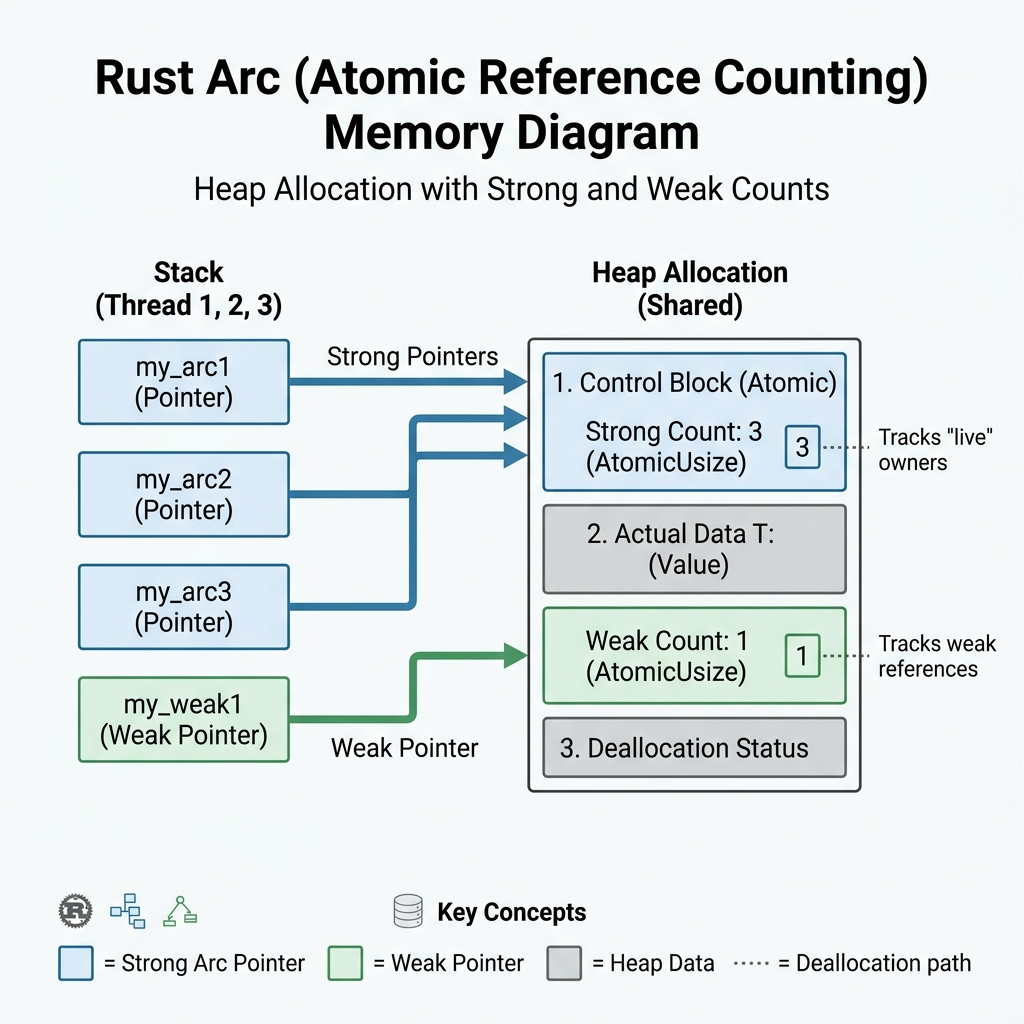
\includegraphics[width=\textwidth]{images/arc_memory.png}
    \caption{Memory layout illustrating Arc atomic reference counting to safely share data across multiple thread boundaries.}
    \label{fig:arc_memory}
\end{figure}

\begin{notebox}
\textbf{Why not use \texttt{Arc<T>} everywhere?} \\
Atomic operations inherently incur a microscopic performance penalty compared to standard integer arithmetic. In purely single-threaded programs, \texttt{Rc<T>} avoids this unnecessary overhead. The Rust compiler actively enforces this logic: it will explicitly refuse to compile if you attempt to send a non-thread-safe \texttt{Rc<T>} across threads!
\end{notebox}

\section{Interior Mutability: \texttt{Cell<T>} and \texttt{RefCell<T>}}
Because \texttt{Rc<T>} and \texttt{Arc<T>} strictly provide shared ownership, they default to immutable access. What happens if a shared variable genuinely needs to be updated? This requires the \textbf{Interior Mutability} pattern, which allows mutating inner data even when external references to that data are strictly immutable.

\subsection{\texttt{Cell<T>}}
\texttt{Cell<T>} facilitates interior mutability by moving values directly in and out of the cell without utilizing pointers. It is designed heavily around lightweight, \texttt{Copy} types. Instead of returning references to the inner value, it strictly copies the value.

\subsection{\texttt{RefCell<T>}}
For complex structures that cannot be cheaply copied, \texttt{RefCell<T>} allows borrowing the inner value immutably or mutably. However, it completely shifts Rust's standard borrow checking from \textit{compile-time} to \textit{runtime}. 

When interacting with a \texttt{RefCell<T>}, you call \texttt{borrow()} for an immutable reference or \texttt{borrow\_mut()} for a mutable one. The \texttt{RefCell} tracks active borrows dynamically during execution. 

\begin{warningbox}
\textbf{Runtime Panics with \texttt{RefCell}} \\
If you violate the golden rule of borrowing (e.g., trying to initiate two mutable borrows simultaneously, or initiating a mutable borrow while immutable borrows exist), \texttt{RefCell<T>} cannot save you at compile-time. Instead, it will instantly \textbf{panic} at runtime, abruptly crashing the thread. 
\end{warningbox}

By cleverly composing \texttt{Rc} and \texttt{RefCell} as \texttt{Rc<RefCell<T>>}, we can achieve both shared ownership and controlled mutability in single-threaded systems.

\begin{exambox}
\textbf{Smart Pointer Matrix for the Exam}
\begin{itemize}
    \item \textbf{\texttt{Box<T>}}: Single owner, mutable or immutable borrow, strictly checked at compile time.
    \item \textbf{\texttt{Rc<T>}}: Multiple shared owners, immutable borrow only, checked at compile time.
    \item \textbf{\texttt{RefCell<T>}}: Single owner, mutable or immutable borrow, dynamically checked at runtime.
    \item \textbf{\texttt{Rc<RefCell<T>>}}: Multiple shared owners, mutable or immutable borrow, dynamically checked at runtime.
\end{itemize}
\end{exambox}

\section*{End-of-Chapter Exam Questions}

\textbf{1. Memory Leaks and Cycle Resolution} \\
Suppose you construct a doubly-linked tree utilizing purely \texttt{Rc<T>}, where a parent node holds an \texttt{Rc} to its children, and children hold an \texttt{Rc} directly pointing back to the parent. Explain at an architectural level why this specific design results in an unrecoverable memory leak when the tree goes out of scope. Propose a structural solution using smart pointers to fix it.

\textbf{2. The \texttt{Rc} vs \texttt{Arc} Trade-off} \\
Why does Rust provide separate standard library types for \texttt{Rc<T>} and \texttt{Arc<T>} rather than simply making \texttt{Rc<T>} thread-safe under the hood? Detail the specific type of undefined behavior that would occur if the compiler permitted sharing an \texttt{Rc<T>} object across concurrent threads.

\textbf{3. Interior Mutability Panics} \\
Explain the fundamental difference between how standard references (\texttt{\&mut T}) and \texttt{RefCell<T>} enforce Rust's borrowing rules. Demonstrate a brief scenario in which using \texttt{RefCell<T>} compiles flawlessly but causes a thread panic in production.
